\section{Methodology}\label{sec:method}

Figure~\ref{fig:selective_residual_framework} illustrates the proposed BotRHG framework. The framework first encodes each account into textual and property representations, then constructs hyperedges from local reference neighbors, and finally applies selective residual correction only to routed accounts with lower local reliability.

\begin{figure}[!htbp]
    \centering
    \includegraphics[width=.88\textwidth]{figures/Architecture.pdf}
    \caption{Framework of BotRHG. The model constructs account representations, builds hyperedges from local reference neighbors, and activates selective residual correction only for routed accounts.}
    \label{fig:selective_residual_framework}
\end{figure}

\subsection{Preliminaries and Problem Formulation}\label{sec:preliminaries}

Let $G_{\mathrm{rel}}=(V,E_{\mathrm{rel}},\mathcal{R},X)$ denote a multi-relation social graph, where $V$ is the account set, $E_{\mathrm{rel}}$ the observed social relations, $\mathcal{R}$ the relation types, and $X\in\mathbb{R}^{|V|\times d}$ the account feature matrix. Each labeled account has $y_i\in\{0,1\}$, where $0$ denotes human and $1$ denotes bot.

We consider a trained base detector $f_{\mathrm{base}}$ that produces an initial posterior $p_i=f_{\mathrm{base}}(x_i,G_{\mathrm{rel}})$, a base prediction $\hat{y}^{(0)}_i=\arg\max_c p_i^{(c)}$, and a low-order representation $x_{\mathrm{low},i}$. Our goal is not to replace the base detector for all accounts, but to identify base predictions with lower local reliability and refine them with higher-order evidence.

\subsection{Feature Encoder}

The feature encoder converts heterogeneous account information into textual and property features.

\paragraph{Textual encoder.}
For each Twitter account, we have access to profile metadata, the self-description, and recent tweets. To obtain a unified user representation compatible with the language model encoder, we linearize these heterogeneous user attributes into a single textual sequence. Specifically, we organize the profile metadata as a profile segment and concatenate it with the description and tweet segments:
\begin{equation}
s_i=\texttt{[P]}\ \mathrm{profile}_i\ \texttt{[D]}\ \mathrm{description}_i\ \texttt{[T]}\ \mathrm{tweets}_i ,
\label{eq:text-sequence}
\end{equation}
Here, \texttt{[P]}, \texttt{[D]}, and \texttt{[T]} denote special segment markers for profile metadata, description, and tweets, respectively. Mentions, hashtags, and URLs are normalized as \texttt{@USER}, \texttt{\#HASHTAG}, and \texttt{HTTPURL}.

\begin{figure}[!htbp]
    \centering
    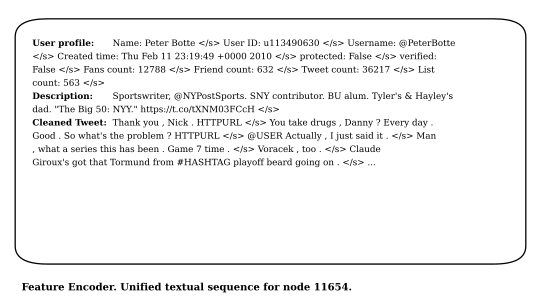
\includegraphics[width=.76\textwidth,trim=75 130 180 60,clip]{figures/feature encoder.pdf}
    \caption{Unified user textual sequence used by the feature encoder.}
    \label{fig:user_text_sequence}
\end{figure}

Following recent language-model-based bot detectors~\cite{cai2024lmbot,zhou2024lgb}, we encode the resulting sequence with a fine-tuned RoBERTa model to obtain the textual representation $h_i^{\mathrm{text}}$, and stack all account representations to form $X^{\mathrm{text}}$.

\paragraph{Property encoder.}
Besides the unified textual sequence, we retain structured user properties to capture account-level and social statistics that are complementary to textual semantics. Following prior bot detection studies~\cite{davis2016botornot,varol2017online,lin2025botbr,gao2025higherorder}, we extract profile, activity, and network-structure attributes from raw user data, and organize them into numerical and categorical feature groups, denoted by $X_{\mathrm{num}}$ and $X_{\mathrm{cat}}$, respectively. Continuous attributes in $X_{\mathrm{num}}$ are normalized with training-split statistics, while categorical and Boolean attributes in $X_{\mathrm{cat}}$ are converted into indicator features. We then project them into latent property representations through two feed-forward layers with LeakyReLU activation $\phi$:
\begin{align}
X_n &= \phi(X_{\mathrm{num}}W_n+b_n),
\label{eq:numerical-property-projection}\\
X_c &= \phi(X_{\mathrm{cat}}W_c+b_c),
\label{eq:categorical-property-projection}
\end{align}
where $W_n$, $W_c$, $b_n$, and $b_c$ are learnable parameters. The initial node feature matrix is
\begin{equation}
X_{\mathrm{in}} = X^{\mathrm{text}} \Vert X_n \Vert X_c ,
\label{eq:node-feature}
\end{equation}
and we denote its $i$-th row by $x_i$.

\subsection{Hypergraph Construction}

To build higher-order evidence, we combine the low-order representation from the base detector with the node feature representation:
\begin{equation}
x_{\mathrm{new},i}=x_{\mathrm{low},i}\Vert x_i .
\label{eq:hybrid-representation}
\end{equation}
Stacking all account representations gives $X_{\mathrm{new}}$, which is used for hypergraph construction.

Let $\mathcal{T}$ denote the target accounts and let $\mathcal{U}_{\mathrm{ref}}$ denote the reference pool used for hypergraph construction and reliability estimation. Following the standard split protocol, reference neighbors are retrieved from the corresponding reference pool, and the target account itself is excluded from its neighborhood. For each target account, we construct a candidate hyperedge from local reference neighbors:
\begin{equation}
e_i=\{i\}\cup \mathcal{N}^{\mathrm{support}}_k(i),\qquad i\in \mathcal{T},
\label{eq:support-hyperedge}
\end{equation}
where $\mathcal{N}^{\mathrm{support}}_k(i)\subseteq \mathcal{U}_{\mathrm{ref}}\setminus\{i\}$ contains the $k$ nearest reference accounts in $X_{\mathrm{new}}$. These target-centered hyperedges provide candidate higher-order evidence for subsequent selective correction.

\subsection{Reliability-Guided Selective Correction}

The correction module is selective: it preserves the base prediction for most accounts and activates higher-order correction only when local reference evidence indicates lower local reliability.

\paragraph{Local reliability estimation.}
Inspired by local reference comparison in conformal-style methods~\cite{vovk2005algorithmic} and selective prediction~\cite{geifman2017selective}, we estimate the reliability of each base prediction relative to similar reference accounts through local reliability estimation inspired by confidence calibration and local reference comparison. We first define the confidence deficit of account $i$ as
\begin{equation}
u_i=1-\max_c p_i^{(c)}.
\label{eq:confidence-deficit}
\end{equation}
For a reference account $j$, let $s_{ij}$ denote the cosine similarity in $X_{\mathrm{new}}$. We convert it to angular distance $d_{ij}=\sqrt{\max(0,2-2s_{ij})}$ and weight $w_{ij}=\exp(-d_{ij}/\lambda)$, where $\lambda=1.0$. The local reference comparison yields
\begin{equation}
\tau_i =
    \frac{1+\sum_{j\in\mathcal{U}_{\mathrm{ref}}\setminus\{i\}} w_{ij}\mathbb{I}[u_j\ge u_i]}
         {1+\sum_{j\in\mathcal{U}_{\mathrm{ref}}\setminus\{i\}} w_{ij}},
\quad
\rho_i = \tau_i,
\quad
r_i = 1-\rho_i .
\label{eq:local-reference-score}
\end{equation}
Eq.~\eqref{eq:local-reference-score} defines the local reliability estimate $\rho_i$ and the corresponding correction risk $r_i$. Accounts that are more uncertain than their local references receive lower reliability and higher correction risk.

\paragraph{Reliability-guided routing.}
Given a routing budget $\beta$, we select
\begin{equation}
B=\lfloor \beta |\mathcal{T}| \rfloor
\label{eq:routing-budget}
\end{equation}
accounts with the highest correction risk:
\begin{align}
R_{\beta} &= \operatorname{TopB}(\{r_i\}_{i\in \mathcal{T}}, B),
\label{eq:routed-set}\\
\mathcal{E}_H^{\beta} &= \{e_i\mid i\in R_{\beta}\}.
\label{eq:routed-hyperedges}
\end{align}
Based on the routing budget in Eq.~\eqref{eq:routing-budget}, Eqs.~\eqref{eq:routed-set} and~\eqref{eq:routed-hyperedges} select the routed account set and the corresponding routed hyperedges. This reliability-guided routing strategy treats higher-order reasoning as a selective intervention, allowing the model to preserve reliable base predictions while concentrating additional correction on low-reliability accounts.

\paragraph{Selective residual correction.}
Let $H\in\{0,1\}^{|V|\times |\mathcal{E}_H^{\beta}|}$ be the incidence matrix of the routed hyperedges. Eqs.~\eqref{eq:hypergraph-initialization} and~\eqref{eq:hypergraph-propagation} compute higher-order representations from $X_{\mathrm{new}}$ through hypergraph propagation:
\begin{align}
X_H^{(0)} &= X_{\mathrm{new}} W_0,
\label{eq:hypergraph-initialization}\\
X_H^{(\ell+1)} &=
\phi\!\left(D_v^{-1/2} H D_e^{-1} H^\top D_v^{-1/2} X_H^{(\ell)} W_{\ell}\right),
\label{eq:hypergraph-propagation}
\end{align}
where $D_v$ and $D_e$ are the node and hyperedge degree matrices, and $\phi(\cdot)$ is a nonlinear activation. The resulting representation is denoted by $x_{\mathrm{high},i}$.

For each routed account, selective residual correction is defined in Eqs.~\eqref{eq:residual-update} and~\eqref{eq:residual-correction} as
\begin{align}
\delta_i &= \psi(x_{\mathrm{low},i}\Vert x_{\mathrm{high},i}),
\label{eq:residual-update}\\
h_i &= x_{\mathrm{low},i}+m_i\delta_i,
\label{eq:residual-correction}
\end{align}
where $\psi$ is a learnable residual projection and $m_i=\mathbb{I}[i\in R_{\beta}]$. The corrected posterior is
\begin{equation}
q_i=\operatorname{softmax}(W_c h_i+b_c),\qquad i\in R_{\beta}.
\label{eq:corrected-posterior}
\end{equation}
The final prediction follows the selective rule in Eq.~\eqref{eq:final-prediction}
\begin{equation}
\hat{y}_i=
\begin{cases}
\arg\max_c q_i^{(c)}, & i\in R_{\beta},\\
\hat{y}^{(0)}_i, & i\notin R_{\beta}.
\end{cases}
\label{eq:final-prediction}
\end{equation}

\subsection{Training and Inference}

Following the standard benchmark split, the base detector is trained with supervised classification and then fixed. During correction training, only the hypergraph branch, the residual projection $\psi$, and the classifier parameters $(W_c,b_c)$ are optimized with cross-entropy on routed training accounts.

At inference time, the fixed base detector produces $p_i$, $\hat{y}^{(0)}_i$, and $x_{\mathrm{low},i}$; hyperedges are constructed from the corresponding reference pool without using target labels; and selective residual correction is applied only to routed accounts, while non-routed accounts retain the base prediction.
